\documentclass[12pt]{article}\usepackage[]{graphicx}\usepackage[]{color}
% maxwidth is the original width if it is less than linewidth
% otherwise use linewidth (to make sure the graphics do not exceed the margin)
\makeatletter
\def\maxwidth{ %
  \ifdim\Gin@nat@width>\linewidth
    \linewidth
  \else
    \Gin@nat@width
  \fi
}
\makeatother

\definecolor{fgcolor}{rgb}{0.345, 0.345, 0.345}
\newcommand{\hlnum}[1]{\textcolor[rgb]{0.686,0.059,0.569}{#1}}%
\newcommand{\hlstr}[1]{\textcolor[rgb]{0.192,0.494,0.8}{#1}}%
\newcommand{\hlcom}[1]{\textcolor[rgb]{0.678,0.584,0.686}{\textit{#1}}}%
\newcommand{\hlopt}[1]{\textcolor[rgb]{0,0,0}{#1}}%
\newcommand{\hlstd}[1]{\textcolor[rgb]{0.345,0.345,0.345}{#1}}%
\newcommand{\hlkwa}[1]{\textcolor[rgb]{0.161,0.373,0.58}{\textbf{#1}}}%
\newcommand{\hlkwb}[1]{\textcolor[rgb]{0.69,0.353,0.396}{#1}}%
\newcommand{\hlkwc}[1]{\textcolor[rgb]{0.333,0.667,0.333}{#1}}%
\newcommand{\hlkwd}[1]{\textcolor[rgb]{0.737,0.353,0.396}{\textbf{#1}}}%
\let\hlipl\hlkwb

\usepackage{framed}
\makeatletter
\newenvironment{kframe}{%
 \def\at@end@of@kframe{}%
 \ifinner\ifhmode%
  \def\at@end@of@kframe{\end{minipage}}%
  \begin{minipage}{\columnwidth}%
 \fi\fi%
 \def\FrameCommand##1{\hskip\@totalleftmargin \hskip-\fboxsep
 \colorbox{shadecolor}{##1}\hskip-\fboxsep
     % There is no \\@totalrightmargin, so:
     \hskip-\linewidth \hskip-\@totalleftmargin \hskip\columnwidth}%
 \MakeFramed {\advance\hsize-\width
   \@totalleftmargin\z@ \linewidth\hsize
   \@setminipage}}%
 {\par\unskip\endMakeFramed%
 \at@end@of@kframe}
\makeatother

\definecolor{shadecolor}{rgb}{.97, .97, .97}
\definecolor{messagecolor}{rgb}{0, 0, 0}
\definecolor{warningcolor}{rgb}{1, 0, 1}
\definecolor{errorcolor}{rgb}{1, 0, 0}
\newenvironment{knitrout}{}{} % an empty environment to be redefined in TeX

\usepackage{alltt}

%%% draft settings

% line numbers
\usepackage{lineno}
\linenumbers

% double spacing
\usepackage{setspace}
\doublespacing

% figures
\usepackage{graphicx}
\usepackage{amsmath,amssymb}

\usepackage{docmute}
\usepackage{tikz}
\usetikzlibrary{shapes, arrows, positioning}
\usepackage{xcolor}
\definecolor{fillgray}{gray}{0.95}
\usepackage{amsmath}

% more words macro
\usepackage[color=lightgray]{todonotes}

\newcommand{\todonote}[1]{
    \todo[inline]{\emph{draft notes} #1}
}

% code
\newcommand{\code}[1]{\texttt{\detokenize{#1}}}
% package
\newcommand{\package}[1]{\texttt{\detokenize{#1::}}}
% function
\newcommand{\function}[1]{\texttt{\detokenize{::#1}}}
% package::function
\newcommand{\pkgfn}[2]{\texttt{\detokenize{#1::#2}}}

% title
\title{A computational way station for reporting network meta-analyses}
\author{Charles T. Gray, Gavin Stewart, Matthew Grainger}
\IfFileExists{upquote.sty}{\usepackage{upquote}}{}
\begin{document}








\todonote{Reminder: don't knit the .TeX file, use .Rnw.}

\section{Reporting standards and Bayesian network meta-analysis}
% manuscript contents

As with many Bayesian algorithms, recent developments in underlying sampling algorithms (such as \code{stan}'s implementation in \code{R}), have enabled advances in Bayesian network meta-analysis (NMA). Software has become available, such as \package{multinma}, released in 2021, which computes Bayesian estimates for NMA using \code{stan} from an \code{R} interface. The key attraction of NMA is how it allows a comparison of multiple treatments, even where direct pairwise comparisons are not empirically available. However, a challenge exists for researchers who wish to both use these techniques and adhere to appropriate evidence synthesis reporting standards for a given discipline. One way of meeting this challenge is to provide a computational waystation for the development of toolchains for reporting NMA according to different standards, such as Cochrane or the Campbell Collaboration. This manuscript provides some toolchain and commentary about the process of computationally implementing a network meta-analysis according to Cochrane's reporting standards and how we might expand our research compendia to include in-development computational science workflows.

\subsection{Network meta-analysis}

Pairwise analyses between treatment and control, exposed and unexposed, intervention and no intervention, are conventionally undertaken with meta-analysis in fields such as ecology, medicine, and the social sciences~\cite{borenstein_introduction_2011}. NMA provides a means of comparing three or more treatments or interventions, including control or placebo~\cite{higgins2019cochrane}. The question answered by an NMA is not \emph{if} a treatment works, but \emph{which} treatments perform better, comparatively~\cite{harrer_doing_2019}. A particularly useful aspect of NMA is combining the results of more than one pairwise analysis and constructing indirect comparisons, where pairwise evidence is unavailable, from a network of direct comparisons. An example of direct comparisons provided by existing evidence is shown in Figure \ref{fig:network}. NMA converts the network to a complete graph, where all treatments are compared with all other treatments, that is, every node connects to every other node via \textbf{direct} or \textbf{indirect} comparison.





\begin{figure}


\begin{knitrout}
\definecolor{shadecolor}{rgb}{0.969, 0.969, 0.969}\color{fgcolor}
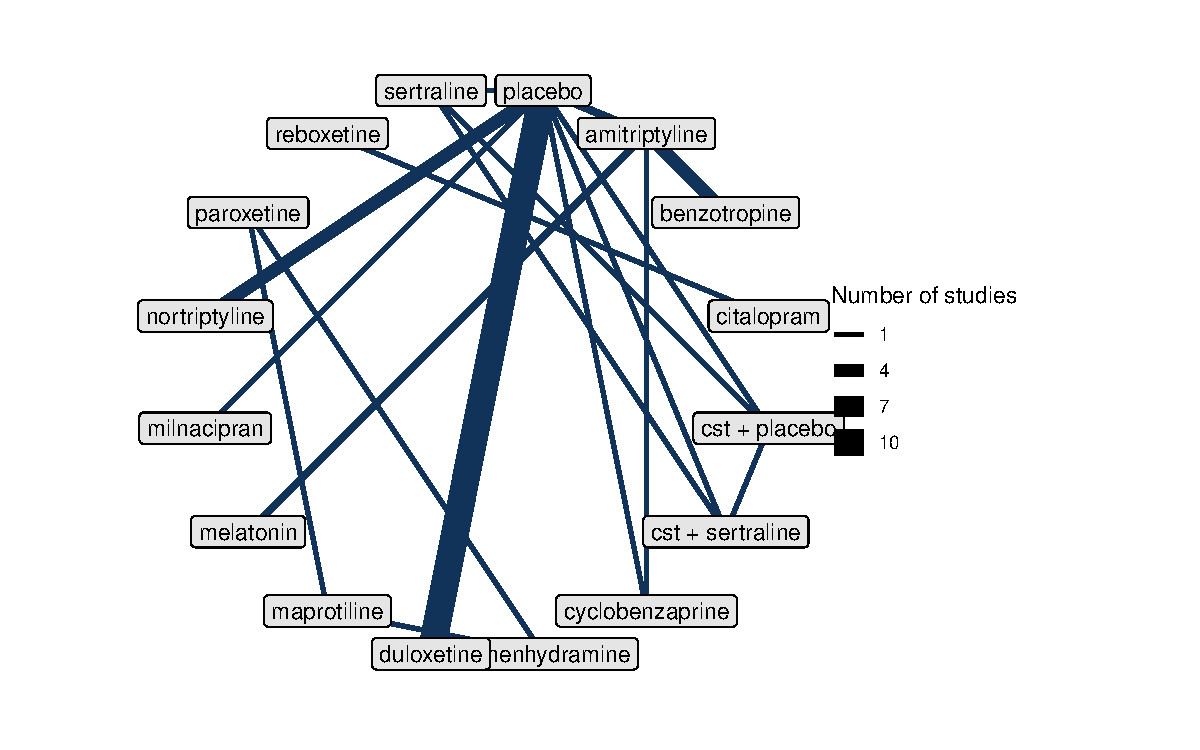
\includegraphics[width=\maxwidth]{figure/network_fig-1} 

\end{knitrout}


\caption{Network of treatment comparisons, the direct evidence, included in the network meta-analysis for how antidepressants affect sleep. This analysis will be discussed in detail in Section \ref{sec:toolchain}, where we describe the data and the toolchains for analysis and reporting.}
\label{fig:network}
\end{figure}

\subsection{Reporting standards}

Reporting NMA according to Cochrane's expectations is a non-trivial task; there are multiple visualisations and tables required, in accordance with standards that have been adapted and derived from existing evidence synthesis standards. Some familiarity with this ecosystem of reporting systems is required to meet the standards required for reporting a NMA according to Cochrane's expectations.

Figure \ref{fig:protocol} shows the immediate development relationships between reporting standards for NMA in Cochrane intervention reviews. A researcher undertaking NMA must ensure they meet (MECIR) and (PRISMA) Extension guidelines, as MECIR was developed for pairwise meta-analysis and the PRISMA Extension provides further guidance on NMA.

\begin{figure}
\centering
\documentclass[draft]{article}
\usepackage[utf8]{inputenc}
\usepackage{tikz}
\usetikzlibrary{shapes, arrows, positioning}
\usepackage{xcolor}
\definecolor{fillgray}{gray}{0.95}
\usepackage{amsmath}


% https://tex.stackexchange.com/questions/168314/how-to-use-latex-commands-to-draw-a-flowchart
\begin{document}

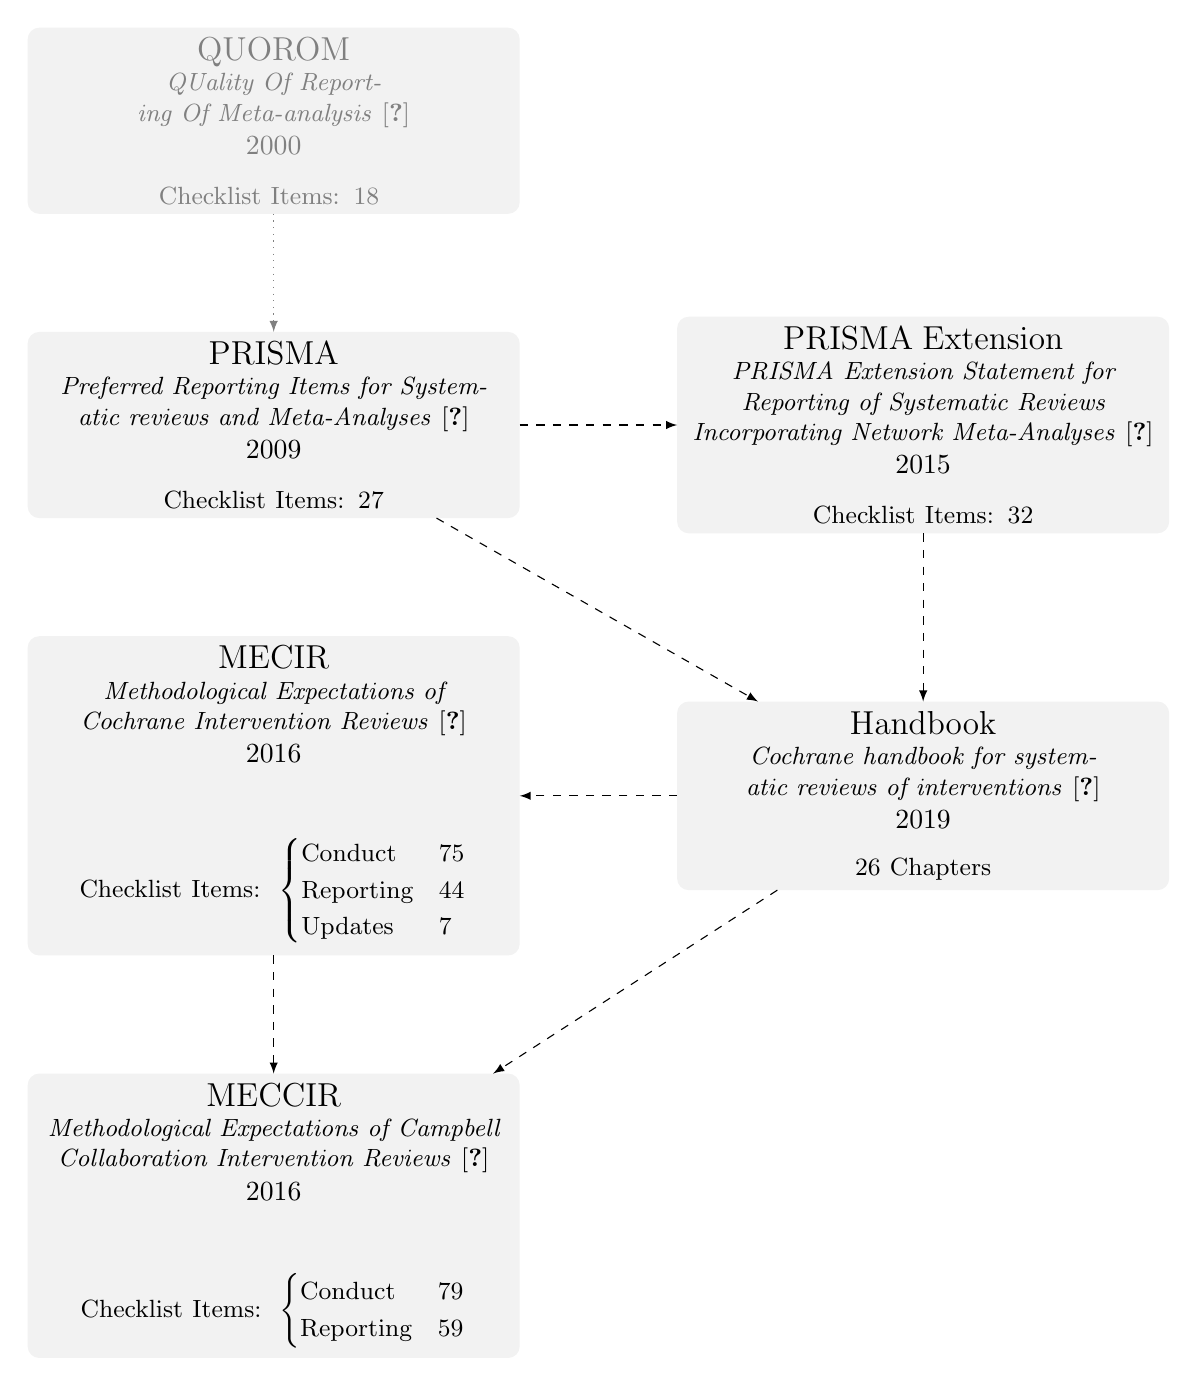
\begin{tikzpicture}[nodes = {
draw=fillgray,
fill=fillgray,
rounded corners,
align=center,
text width=6cm
},
node distance=4cm,
arrows = {-latex}]

% protocols
\node (QUOROM)  {
\textcolor{gray}{
\large{QUOROM}\\
\small{\emph{QUality Of Reporting Of Meta-analysis}~\cite{moher_improving_1999}}\\
\normalsize{2000}\\
\medskip
\small{Checklist Items: 18}
}
};
\node (PRISMA) [below = 1.5cm of QUOROM] {
\large{PRISMA}\\
\small{\emph{Preferred Reporting Items for Systematic reviews and Meta-Analyses}~\cite{liberati_prisma_2009}}\\
\normalsize{2009}\\
\medskip

\small{Checklist Items: 27}
};
\node (MECIR) [below = 1.5cm of PRISMA] {
\large{MECIR}\\
\small{\emph{Methodological Expectations of Cochrane Intervention Reviews}~\cite{higgins_methodological_2016}}\\
\normalsize{2016}\\
\medskip

\small{
\[
\text{Checklist Items: }
\begin{cases}
\text{Conduct} & 75\\
\text{Reporting} & 44\\
\text{Updates} & 7
\end{cases}
\]
}
};
\node (PRISMAext) [right =2cm of PRISMA] {
\large{PRISMA Extension}\\
\small{\emph{PRISMA Extension Statement for Reporting of Systematic Reviews Incorporating Network Meta-Analyses}~\cite{hutton_prisma_2015}}\\
\normalsize{2015}\\
\medskip
\small{Checklist Items: 32}
};

\node (handbook) [right = 2cm of MECIR] {
\large{Handbook}\\
\small{\emph{Cochrane handbook for systematic reviews of interventions}~\cite{higgins2019cochrane}}\\
\normalsize{2019}\\
\medskip
\small{26 Chapters}

};

\node (MECCIR) [below = 1.5cm of MECIR] {
\large{MECCIR}\\
\small{\emph{Methodological Expectations of Campbell Collaboration Intervention Reviews}~\cite{noauthor_campbell_2014}}\\
\normalsize{2016}\\
\medskip

\small{
\[
\text{Checklist Items: }
\begin{cases}
\text{Conduct} & 79\\
\text{Reporting} & 59
\end{cases}
\]
}

};


% connections
\draw [dotted, gray] (QUOROM) to (PRISMA);
\draw  [dashed] (PRISMA) to (PRISMAext);
\draw [dashed] (PRISMA) to (handbook);
\draw  [dashed](PRISMAext) to (handbook);
\draw [dashed] (handbook) to (MECIR);
\draw [dashed] (MECIR) to (MECCIR);
\draw [dashed] (handbook) to (MECCIR);

\end{tikzpicture}

%\bibliographystyle{plain}
%\bibliography{wileyNJD-AMA}

\end{document}

\caption{Development network in which reporting protocols for NMA in Cochrane intervention reviews have been developed.} \label{fig:protocol}
\end{figure}

This figure also provides further information, to demonstrate different ways a researcher may encounter reporting standards. (QUOROM) guidelines have been superseded by PRISMA, from which MECIR was developed. If a researcher is undertaking a Campbell systematic review, they will consult (MECCIR), which was derived from MECIR. MECIR was derived from the Cochrane Handbook, which was informed by PRISMA guidelines.

\section{Toolchains for NMA reporting}
\label{sec:toolchain}

To illustrate the computational challenges of reporting results using newer statistical methods, we step through providing reporting NMA results for a single analysis from an in-development Cochrane intervention review. Before discussing the codeflow in detail, we describe the data analysed.

\subsection{Antidepressants for chronic pain in adults}

These data are a preliminary subset of results from a currently underway Cochrane study examining the use of antidepressants to treat chronic pain in adults.

\todonote{Cite protocol}

These data are intended to be computationally illustrative only, as results and models are not fully developed and only reflect half of the extraction to be completed.

\begin{table}
\caption{Number of observations we have, and of some types we care about in this analysis.}
\label{tab:obs}



\end{table}

\todonote{May need to update this if I change datasets}

In addition to pain, the study examines other ways individuals are affected by chronic pain, such as depression and quality of life. These data present measures of insomnia experienced by chronic pain, with pairwise comparisons between antidepressant interventions and placebo groups.




\todonote{Discuss number of studies and other characterists, treatments, dosages, etc.}


\subsection{Toolchain for reporting the results of one outcome}


In this section we focus on computationally achieving mandatory MECIR reporting for effects and interventions (R76-R99)~\cite{higgins_methodological_2016} on the sleep dataset described above. The examples provided are selected to demonstrate the challenges and nuances of reporting NMA according to MECIR in R.

\todonote{Discuss with Gav how this relates to MECIR; which reporting protocols to include, R76-99?}

\subsubsection{Number of studies and participants: R78}

% gt with spanners
% contribution matrix

To meet this expectation, we need to \emph{state how many studies and how many participants contributed data to results for each outcome, along with the proportion of included studies}. This can be achieved with a summary table with a \textbf{contribution matrix}, which shows the proportions of studies' direct evidence contributions to the treatment comparisons.

\todonote{Is this how to interpret this reporting standard?}

\subsubsection{Estimated outcomes and associated uncertainty (R82-84, R88, R93, R95)}

% forest plot

Outcome effect estimates need to be provided (R82), along with a measure (R82) of uncertainty (we will use confidence interval) with a specified level of confidence, instead of p-values (R84)~\cite{higgins_methodological_2016}. The direction (R88) of the results also needs to be reported. Much of this can be achieved with a forest plot (R93) with appropriate labels (R95) and a table.

\subsubsection{Sensitivity analysis (R94)}

% threshold analysis

Multiple sensitivity analyses should be presented in summary form, not multiple forest plots (R94)~\cite{higgins_methodological_2016}. A threshold analysis is not only a convenient way to summarise multiple sensitivity analyses, but more robust~\cite{phillippo_threshold_2019}.

% \subsubsection{Summary of findings table (R98)}

% gt with spanners


\section{Role of computational waystations}

The toolchain in Section \ref{sec:toolchain} demonstrates the computational gap between statistical methodology and reporting implementation according to a particular protocol. Even where there are well-featured software tools, such as \package{multinma}, different reporting protocols for particular disciplines across which a statistical methodology may be applied will have different requirements. Thus it is unsurprising that for recently-developed statistical methodology there are toolchain gaps that an applied scientist will need to bridge. Computational waystations provide an open science forum in which to develop toolchains, share knowledge, and extend on existing tools.

\bibliographystyle{plain}
\bibliography{references}

\end{document}
